% Options for packages loaded elsewhere
\PassOptionsToPackage{unicode}{hyperref}
\PassOptionsToPackage{hyphens}{url}
%
\documentclass[
  ngerman,
  ignorenonframetext,
]{beamer}
\usepackage{pgfpages}
\setbeamertemplate{caption}[numbered]
\setbeamertemplate{caption label separator}{: }
\setbeamercolor{caption name}{fg=normal text.fg}
\beamertemplatenavigationsymbolsempty
% Prevent slide breaks in the middle of a paragraph
\widowpenalties 1 10000
\raggedbottom
\setbeamertemplate{part page}{
  \centering
  \begin{beamercolorbox}[sep=16pt,center]{part title}
    \usebeamerfont{part title}\insertpart\par
  \end{beamercolorbox}
}
\setbeamertemplate{section page}{
  \centering
  \begin{beamercolorbox}[sep=12pt,center]{part title}
    \usebeamerfont{section title}\insertsection\par
  \end{beamercolorbox}
}
\setbeamertemplate{subsection page}{
  \centering
  \begin{beamercolorbox}[sep=8pt,center]{part title}
    \usebeamerfont{subsection title}\insertsubsection\par
  \end{beamercolorbox}
}
\AtBeginPart{
  \frame{\partpage}
}
\AtBeginSection{
  \ifbibliography
  \else
    \frame{\sectionpage}
  \fi
}
\AtBeginSubsection{
  \frame{\subsectionpage}
}
\usepackage{amsmath,amssymb}
\usepackage{lmodern}
\usepackage{iftex}
\ifPDFTeX
  \usepackage[T1]{fontenc}
  \usepackage[utf8]{inputenc}
  \usepackage{textcomp} % provide euro and other symbols
\else % if luatex or xetex
  \usepackage{unicode-math}
  \defaultfontfeatures{Scale=MatchLowercase}
  \defaultfontfeatures[\rmfamily]{Ligatures=TeX,Scale=1}
\fi
\usetheme[]{Berkeley}
% Use upquote if available, for straight quotes in verbatim environments
\IfFileExists{upquote.sty}{\usepackage{upquote}}{}
\IfFileExists{microtype.sty}{% use microtype if available
  \usepackage[]{microtype}
  \UseMicrotypeSet[protrusion]{basicmath} % disable protrusion for tt fonts
}{}
\makeatletter
\@ifundefined{KOMAClassName}{% if non-KOMA class
  \IfFileExists{parskip.sty}{%
    \usepackage{parskip}
  }{% else
    \setlength{\parindent}{0pt}
    \setlength{\parskip}{6pt plus 2pt minus 1pt}}
}{% if KOMA class
  \KOMAoptions{parskip=half}}
\makeatother
\usepackage{xcolor}
\IfFileExists{xurl.sty}{\usepackage{xurl}}{} % add URL line breaks if available
\IfFileExists{bookmark.sty}{\usepackage{bookmark}}{\usepackage{hyperref}}
\hypersetup{
  pdftitle={Thema 2: Bayes-Modelle einer kleinen Welt},
  pdfauthor={Prof.~Sauer},
  pdflang={de-DE},
  hidelinks,
  pdfcreator={LaTeX via pandoc}}
\urlstyle{same} % disable monospaced font for URLs
\newif\ifbibliography
\usepackage{color}
\usepackage{fancyvrb}
\newcommand{\VerbBar}{|}
\newcommand{\VERB}{\Verb[commandchars=\\\{\}]}
\DefineVerbatimEnvironment{Highlighting}{Verbatim}{commandchars=\\\{\}}
% Add ',fontsize=\small' for more characters per line
\usepackage{framed}
\definecolor{shadecolor}{RGB}{248,248,248}
\newenvironment{Shaded}{\begin{snugshade}}{\end{snugshade}}
\newcommand{\AlertTok}[1]{\textcolor[rgb]{0.94,0.16,0.16}{#1}}
\newcommand{\AnnotationTok}[1]{\textcolor[rgb]{0.56,0.35,0.01}{\textbf{\textit{#1}}}}
\newcommand{\AttributeTok}[1]{\textcolor[rgb]{0.77,0.63,0.00}{#1}}
\newcommand{\BaseNTok}[1]{\textcolor[rgb]{0.00,0.00,0.81}{#1}}
\newcommand{\BuiltInTok}[1]{#1}
\newcommand{\CharTok}[1]{\textcolor[rgb]{0.31,0.60,0.02}{#1}}
\newcommand{\CommentTok}[1]{\textcolor[rgb]{0.56,0.35,0.01}{\textit{#1}}}
\newcommand{\CommentVarTok}[1]{\textcolor[rgb]{0.56,0.35,0.01}{\textbf{\textit{#1}}}}
\newcommand{\ConstantTok}[1]{\textcolor[rgb]{0.00,0.00,0.00}{#1}}
\newcommand{\ControlFlowTok}[1]{\textcolor[rgb]{0.13,0.29,0.53}{\textbf{#1}}}
\newcommand{\DataTypeTok}[1]{\textcolor[rgb]{0.13,0.29,0.53}{#1}}
\newcommand{\DecValTok}[1]{\textcolor[rgb]{0.00,0.00,0.81}{#1}}
\newcommand{\DocumentationTok}[1]{\textcolor[rgb]{0.56,0.35,0.01}{\textbf{\textit{#1}}}}
\newcommand{\ErrorTok}[1]{\textcolor[rgb]{0.64,0.00,0.00}{\textbf{#1}}}
\newcommand{\ExtensionTok}[1]{#1}
\newcommand{\FloatTok}[1]{\textcolor[rgb]{0.00,0.00,0.81}{#1}}
\newcommand{\FunctionTok}[1]{\textcolor[rgb]{0.00,0.00,0.00}{#1}}
\newcommand{\ImportTok}[1]{#1}
\newcommand{\InformationTok}[1]{\textcolor[rgb]{0.56,0.35,0.01}{\textbf{\textit{#1}}}}
\newcommand{\KeywordTok}[1]{\textcolor[rgb]{0.13,0.29,0.53}{\textbf{#1}}}
\newcommand{\NormalTok}[1]{#1}
\newcommand{\OperatorTok}[1]{\textcolor[rgb]{0.81,0.36,0.00}{\textbf{#1}}}
\newcommand{\OtherTok}[1]{\textcolor[rgb]{0.56,0.35,0.01}{#1}}
\newcommand{\PreprocessorTok}[1]{\textcolor[rgb]{0.56,0.35,0.01}{\textit{#1}}}
\newcommand{\RegionMarkerTok}[1]{#1}
\newcommand{\SpecialCharTok}[1]{\textcolor[rgb]{0.00,0.00,0.00}{#1}}
\newcommand{\SpecialStringTok}[1]{\textcolor[rgb]{0.31,0.60,0.02}{#1}}
\newcommand{\StringTok}[1]{\textcolor[rgb]{0.31,0.60,0.02}{#1}}
\newcommand{\VariableTok}[1]{\textcolor[rgb]{0.00,0.00,0.00}{#1}}
\newcommand{\VerbatimStringTok}[1]{\textcolor[rgb]{0.31,0.60,0.02}{#1}}
\newcommand{\WarningTok}[1]{\textcolor[rgb]{0.56,0.35,0.01}{\textbf{\textit{#1}}}}
\setlength{\emergencystretch}{3em} % prevent overfull lines
\providecommand{\tightlist}{%
  \setlength{\itemsep}{0pt}\setlength{\parskip}{0pt}}
\setcounter{secnumdepth}{5}
%\setbeamertemplate{page number in head/foot}[totalframenumber]
\setbeamertemplate{footline}[frame number]
\ifXeTeX
  % Load polyglossia as late as possible: uses bidi with RTL langages (e.g. Hebrew, Arabic)
  \usepackage{polyglossia}
  \setmainlanguage[]{german}
\else
  \usepackage[main=ngerman]{babel}
% get rid of language-specific shorthands (see #6817):
\let\LanguageShortHands\languageshorthands
\def\languageshorthands#1{}
\fi
\ifLuaTeX
  \usepackage{selnolig}  % disable illegal ligatures
\fi
\newlength{\cslhangindent}
\setlength{\cslhangindent}{1.5em}
\newlength{\csllabelwidth}
\setlength{\csllabelwidth}{3em}
\newenvironment{CSLReferences}[2] % #1 hanging-ident, #2 entry spacing
 {% don't indent paragraphs
  \setlength{\parindent}{0pt}
  % turn on hanging indent if param 1 is 1
  \ifodd #1 \everypar{\setlength{\hangindent}{\cslhangindent}}\ignorespaces\fi
  % set entry spacing
  \ifnum #2 > 0
  \setlength{\parskip}{#2\baselineskip}
  \fi
 }%
 {}
\usepackage{calc}
\newcommand{\CSLBlock}[1]{#1\hfill\break}
\newcommand{\CSLLeftMargin}[1]{\parbox[t]{\csllabelwidth}{#1}}
\newcommand{\CSLRightInline}[1]{\parbox[t]{\linewidth - \csllabelwidth}{#1}\break}
\newcommand{\CSLIndent}[1]{\hspace{\cslhangindent}#1}
\usepackage{csquotes}

\title{Thema 2: Bayes-Modelle einer kleinen Welt}
\subtitle{QM2, ReThink, Kap. 2}
\author{Prof.~Sauer}
\date{WiSe 21}
\institute{AWM, HS Ansbach}

\begin{document}
\frame{\titlepage}

\begin{frame}[allowframebreaks]
  \tableofcontents[hideallsubsections]
\end{frame}
\hypertarget{kleine-welt-grouxdfe-welt}{%
\section{Kleine Welt, große Welt}\label{kleine-welt-grouxdfe-welt}}

\begin{frame}{Behaims Globus, Kolumbus glücklicher Fehler}
\protect\hypertarget{behaims-globus-kolumbus-gluxfccklicher-fehler}{}
\begin{figure}[H]
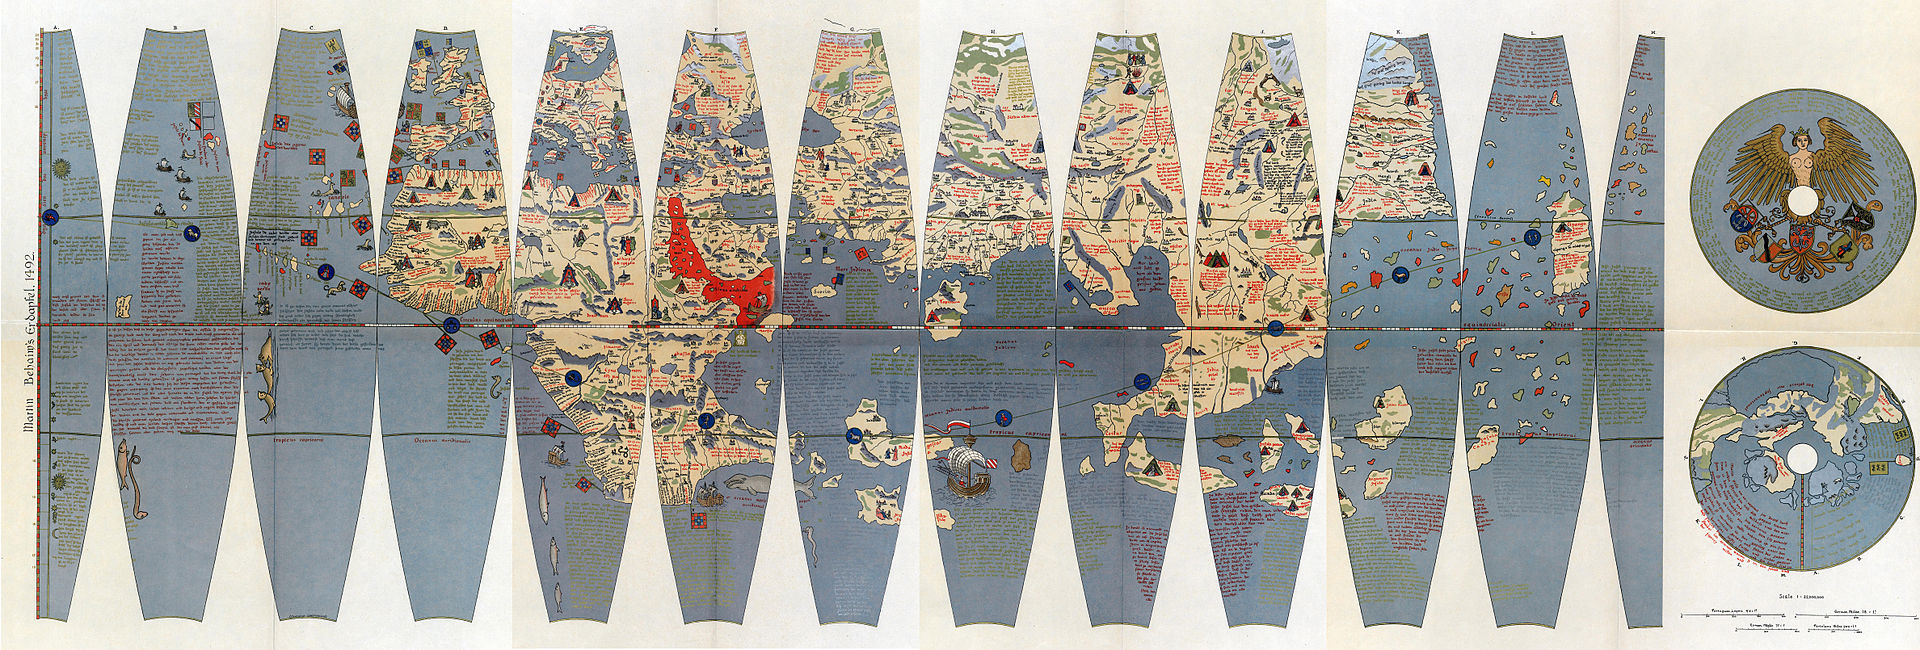
\includegraphics[width=1\linewidth]{/Users/sebastiansaueruser/github-repos/QM2-Folien/img/Behaim} \end{figure}

\href{https://de.wikipedia.org/wiki/Martin_Behaims_Erdapfel\#/media/Datei:RavensteinBehaim.jpg}{Quelle}
\end{frame}

\begin{frame}{Kleine Welt, große Welt}
\protect\hypertarget{kleine-welt-grouxdfe-welt-1}{}
\begin{columns}[T]
\begin{column}{0.5\textwidth}
\begin{block}{Kleine Welt}
\protect\hypertarget{kleine-welt}{}
\begin{itemize}
\tightlist
\item
  Die Welt, wie sie der Golem sieht
\item
  entspricht dem Modell (zwangläufig)
\end{itemize}
\end{block}
\end{column}

\begin{column}{0.5\textwidth}
\begin{block}{Große Welt}
\protect\hypertarget{grouxdfe-welt}{}
\begin{itemize}
\tightlist
\item
  Die Welt, wie sie in Wirklichkeit ist
\item
  entspricht nicht (zwangsläufig) dem Modell
\end{itemize}
\end{block}
\end{column}
\end{columns}

\begin{itemize}
\tightlist
\item
  Die kleine Welt ist nicht die große Welt.
\item
  Was in der kleinen Welt funktioniert, muss nicht in der großen Welt
  funktionieren.
\item
  Modelle zeigen immer nur die kleine Welt: Vorsicht vor schnellen
  Schlüssen und vermeintlicher Gewissheit.
\end{itemize}


\includegraphics[width=1em]{../img/weight.pdf} Nennen Sie ein Beispiel,
in dem ein Modell nicht (exakt) der Wirklichkeit entspricht!
\end{frame}

\begin{frame}{So denkt unser Bayes-Golem}
\protect\hypertarget{so-denkt-unser-bayes-golem}{}
\begin{figure}[H]

\includegraphics[width=1\linewidth]{/Users/sebastiansaueruser/github-repos/QM2-Folien/img/bayesupdate2} \end{figure}


\includegraphics[width=1em]{../img/weight.pdf} Bayes-Inferenz ähnelt dem
Lernen von Menschen. Geben Sie ein Beispiel von Lernen bei Menschen, das
oben dargestelltem Prozess ähnelt!
\end{frame}

\hypertarget{bayes-statistik-als-zuxe4hlen}{%
\section{Bayes-Statistik als
Zählen}\label{bayes-statistik-als-zuxe4hlen}}

\begin{frame}{Murmeln im Säckchen}
\protect\hypertarget{murmeln-im-suxe4ckchen}{}
\begin{itemize}
\item
  Sie haben ein Säckchen mit vier Murmeln darin.
\item
  Sie wissen nicht, welche Farben die Murmeln haben.
\item
  Murmeln gibt's in zwei Farben: weiß (W) oder blau (B).
\item
  Es gibt daher fünf \emph{Hypothesen} zur Farbe der Murmeln im
  Säckchen: {[}WWWW{]}, {[}BWWW{]}, {[}BBWW{]}, {[}BBBW{]}, {[}BBBB.{]}
\item
  Unser Ziel ist, die Wahrscheinlichkeiten der Hypothesen nach Ziehen
  von Murmeln zu bestimmen.
\end{itemize}

\begin{figure}[H]
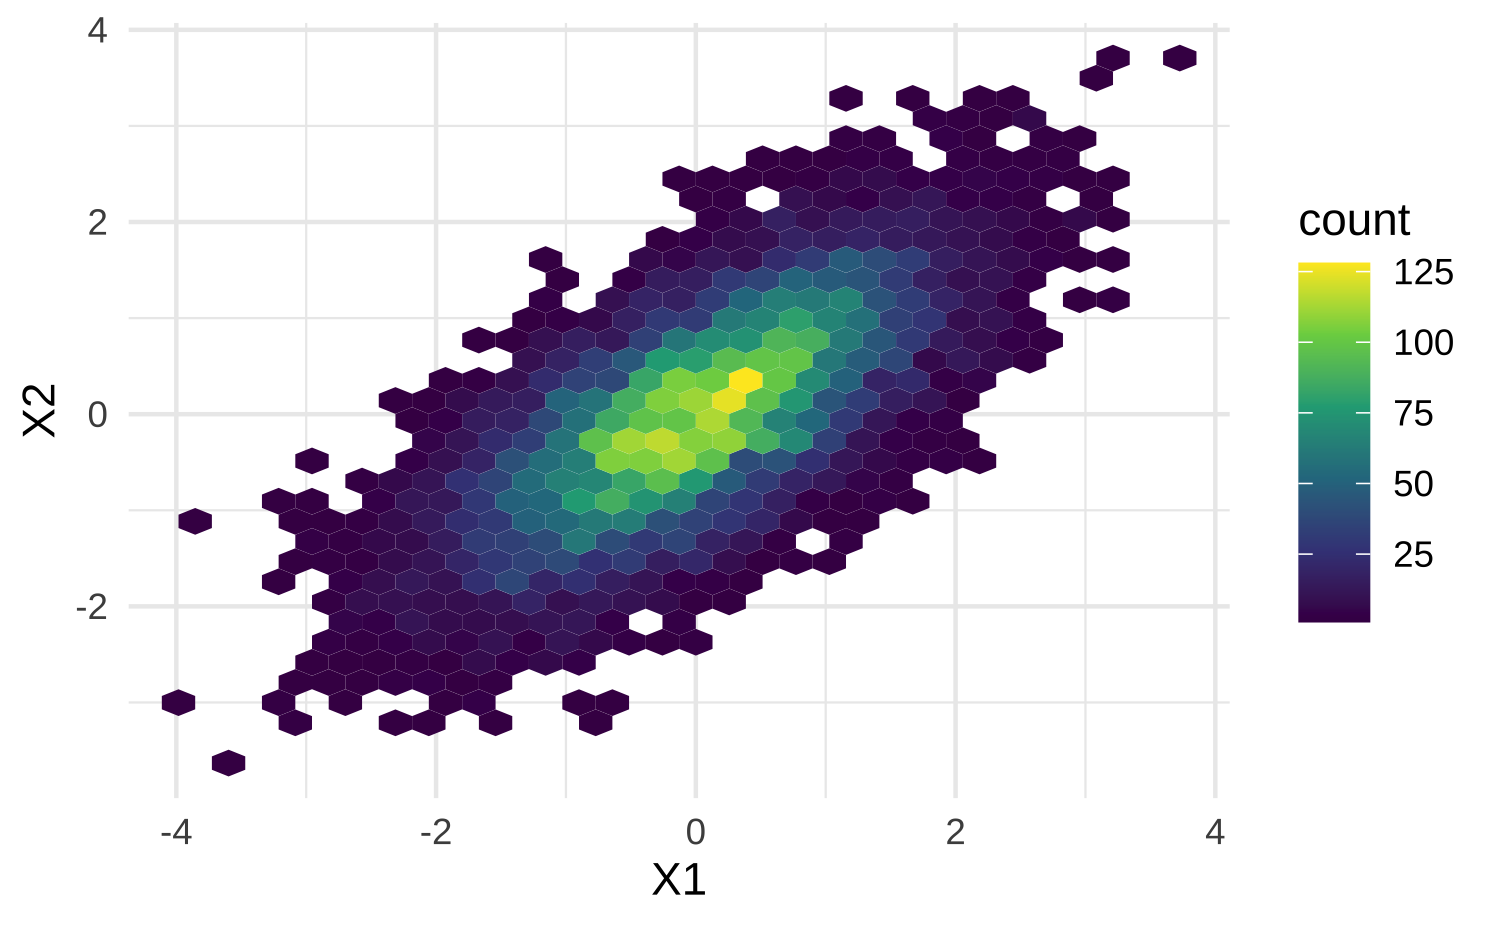
\includegraphics[width=0.5\linewidth]{unnamed-chunk-6-1} \end{figure}
\end{frame}

\begin{frame}{Unsere Daten}
\protect\hypertarget{unsere-daten}{}
\begin{itemize}
\item
  Wir ziehen eine Murmel, merken uns die Farbe und legen sie zurück. Das
  wiederholen wir noch zwei Mal (Ziehen mit Zurücklegen).
\item
  Wir erhalten: \textbf{BWB}. Voilà: unsere Daten.
\end{itemize}

\begin{figure}[H]
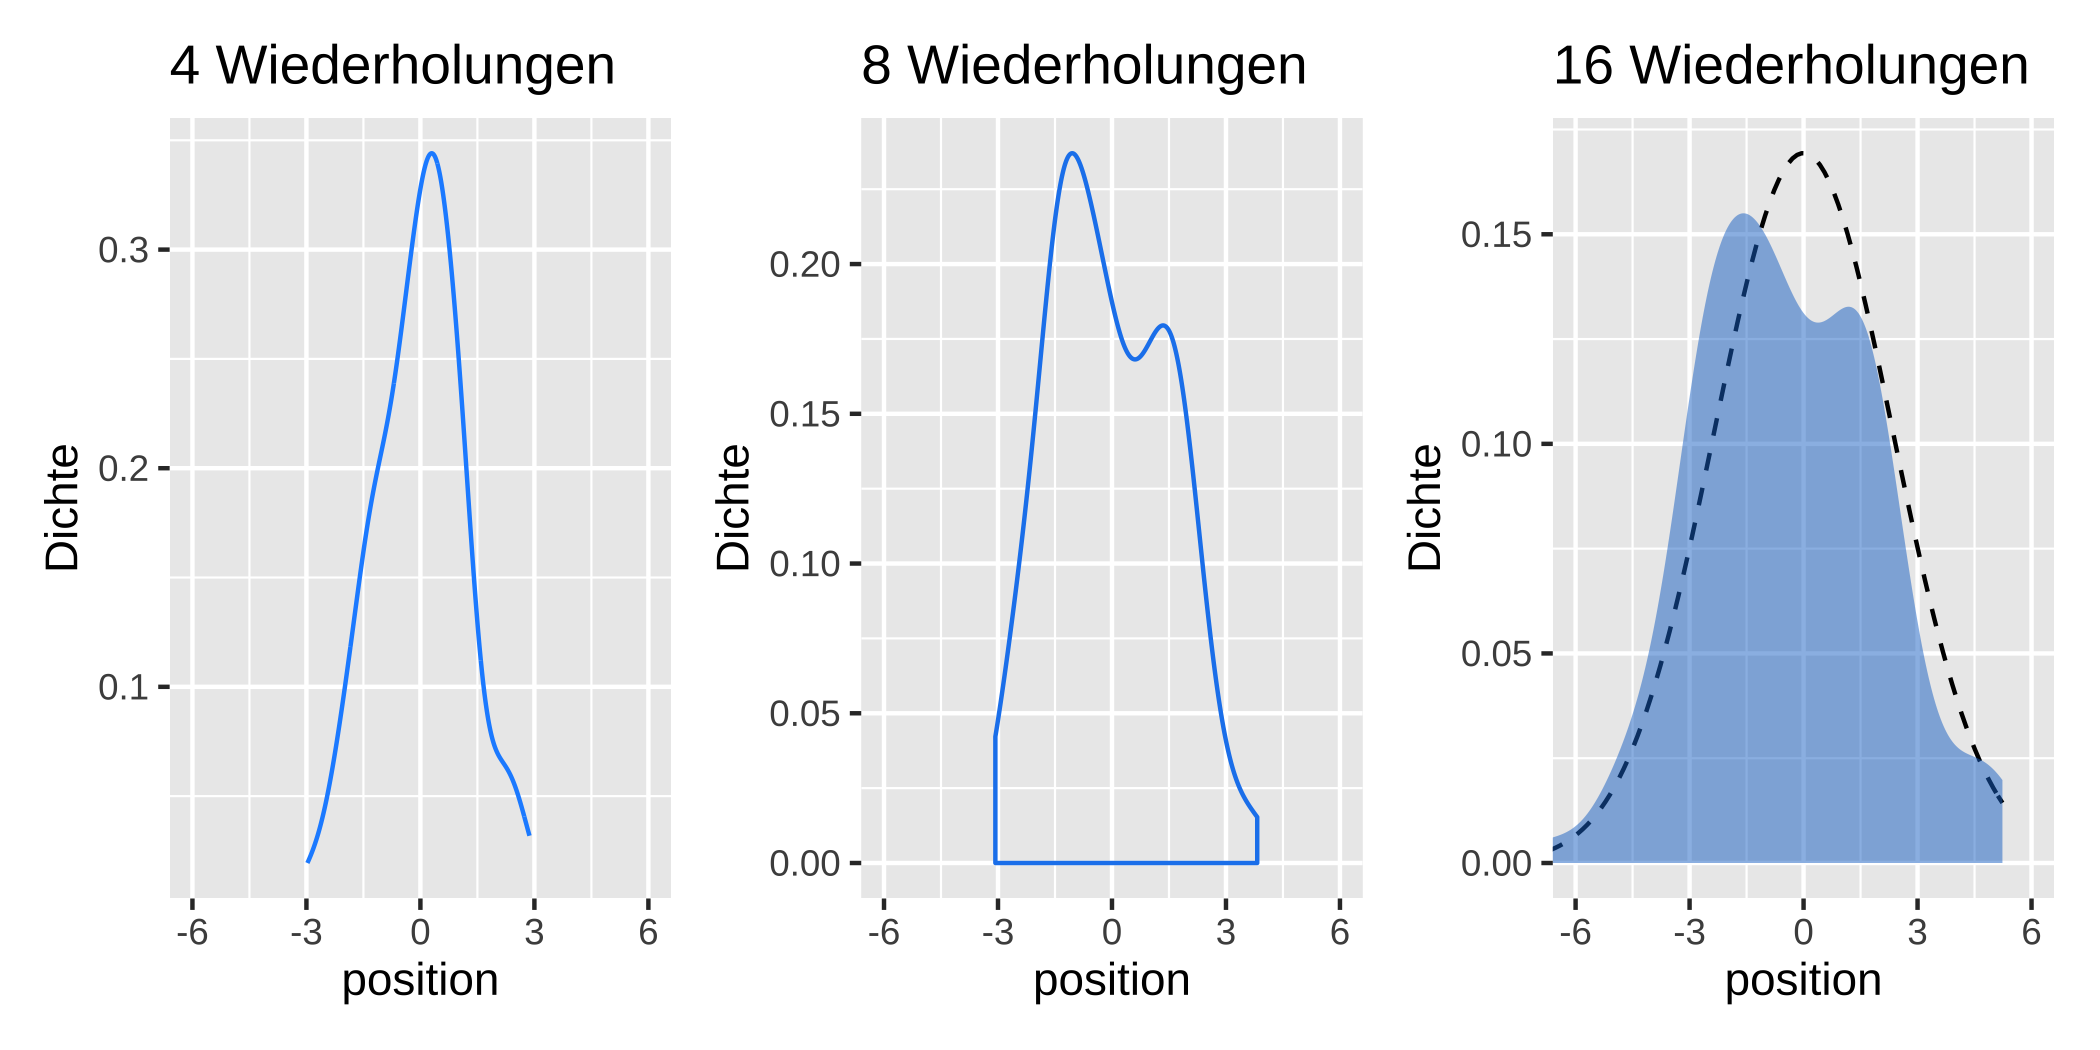
\includegraphics[width=0.7\linewidth]{unnamed-chunk-7-1} \end{figure}

(Kurz 2021)


\includegraphics[width=1em]{../img/weight.pdf} Wie groß ist die
Stichprobe (\(N\))? Ist die Wahrscheinlichkeit für \emph{B} in jedem Zug
gleich?
\end{frame}

\begin{frame}{Zugmöglichkeiten laut Hypothese {[}BWWW{]}, 1. Zug}
\protect\hypertarget{zugmuxf6glichkeiten-laut-hypothese-bwww-1.-zug}{}
Wenn Hypothese {[}BWWW{]} der Fall sein sollte, dann können wir im
\emph{ersten} Zug entweder die eine blaue Murmel erwischen oder eine der
drei weißen.

\begin{figure}[H]
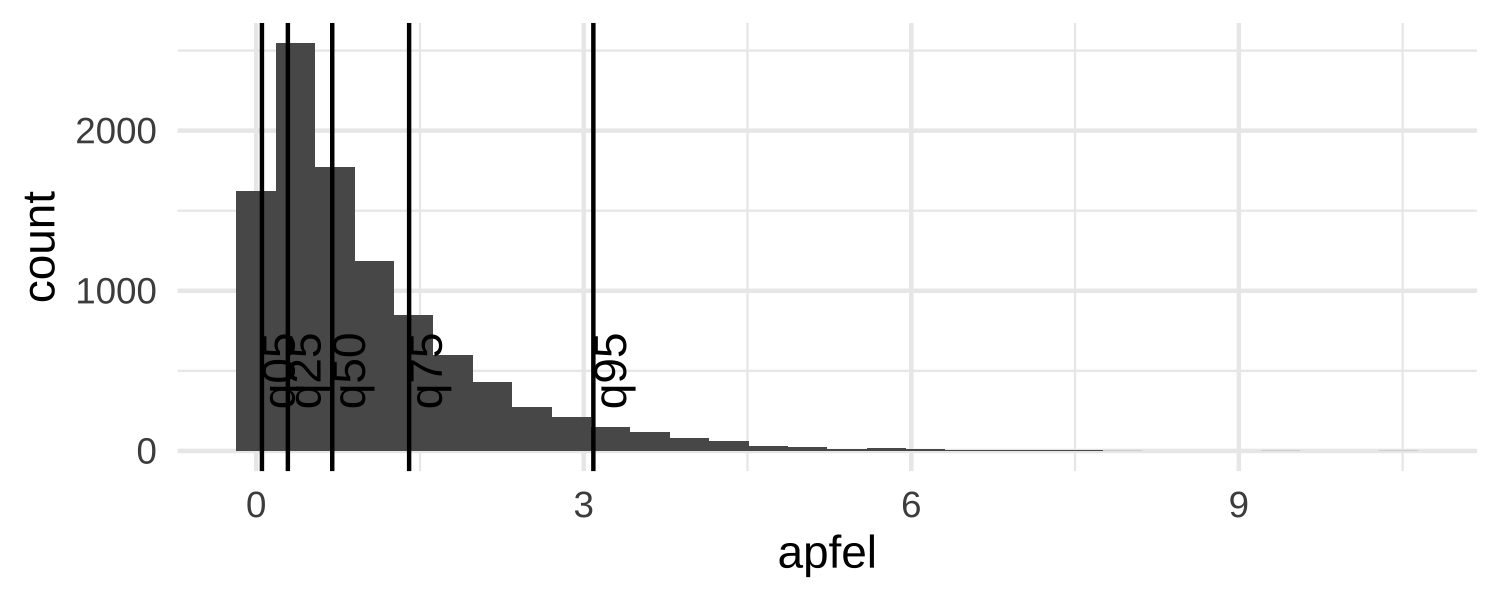
\includegraphics[width=0.7\linewidth]{unnamed-chunk-8-1} \end{figure}

Nachdem wir die Murmel gezogen haben (und die Farbe gemerkt haben),
legen wir sie wieder ins Säckchen: Ziehen mit Zurücklegen.


\includegraphics[width=1em]{../img/weight.pdf} Wie viele
Elementarereignisse hat dieses Zufallsexperiment? Sind alle gleich
wahrscheinlich?
\end{frame}

\begin{frame}{Zugmöglichkeiten laut Hypothese {[}BWWW{]}, 1. und 2. Zug}
\protect\hypertarget{zugmuxf6glichkeiten-laut-hypothese-bwww-1.-und-2.-zug}{}
Wenn Hypothese {[}BWWW{]} der Fall sein sollte, dann haben wir im
\emph{zweiten} Zug natürlich die gleichen Möglichkeiten wie im ersten.

Zug 1 und Zug 2 zusammen genommen gibt es \(16=4\cdot4=4^2\)
Kombinationen an gezogenen Murmeln:

\begin{figure}[H]
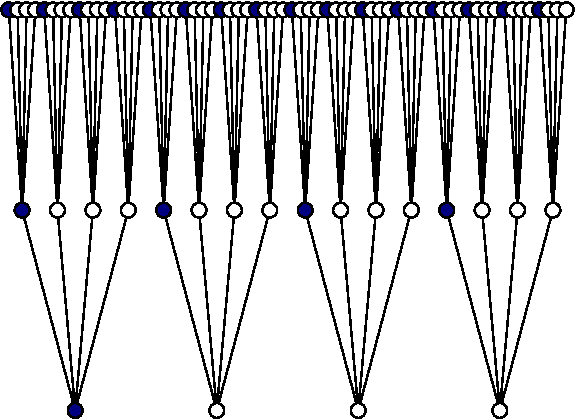
\includegraphics[width=0.5\linewidth]{unnamed-chunk-9-1} \end{figure}


\includegraphics[width=1em]{../img/weight.pdf} Ist jedes
Elementarereignis (z.B. BB, BW,\ldots) gleich wahrscheinlich?
\end{frame}

\begin{frame}{Zugmöglichkeiten laut Hypothese {[}BWWW{]}, 1.-3. Zug}
\protect\hypertarget{zugmuxf6glichkeiten-laut-hypothese-bwww-1.-3.-zug}{}
Zug 1, Zug 2 und Zug 3 zusammen genommen, gibt es dann
\(4\cdot4\cdot4=4^3=64\) Kombinationen, drei Murmeln zu ziehen.

\begin{figure}[H]
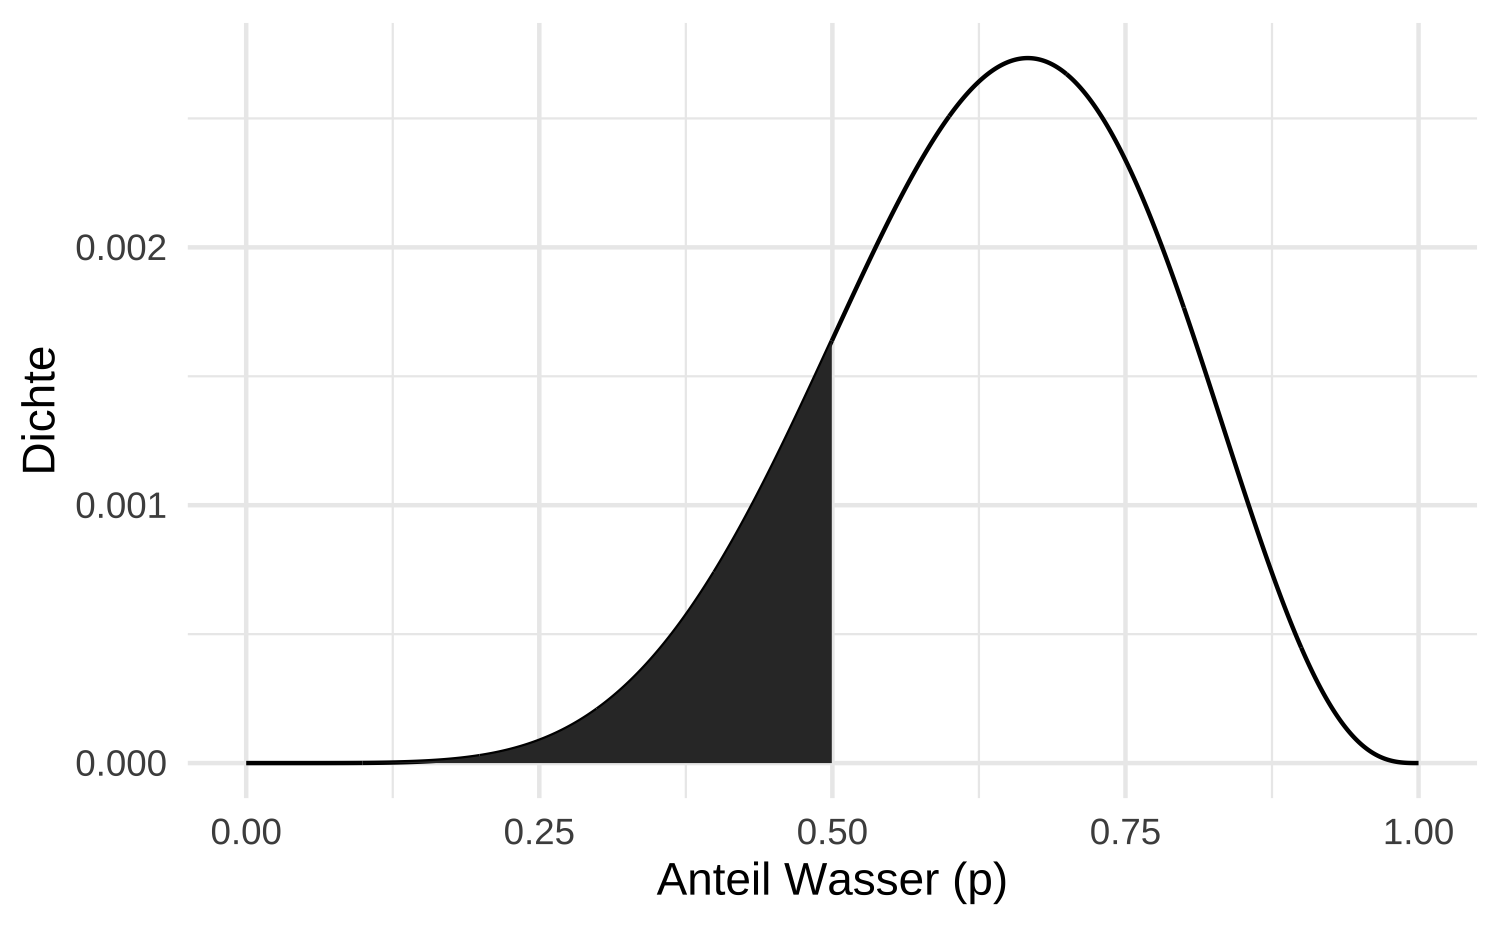
\includegraphics[width=0.5\linewidth]{unnamed-chunk-10-1} \end{figure}


\includegraphics[width=1em]{../img/weight.pdf} Wie wahrscheinlich ist
ein bestimmtes dieser 64 Ereignisse (unter der Annahme gleicher
Wahrscheinlichkeit)?
\end{frame}

\begin{frame}{Welche Züge sind logisch möglich?}
\protect\hypertarget{welche-zuxfcge-sind-logisch-muxf6glich}{}
\begin{itemize}
\tightlist
\item
  Einige Kombinationen (\enquote{Pfade}) der Hypothese {[}BWWW{]} lassen
  sich nicht mit unseren Daten (BWB) vereinbaren.
\item
  Z.B. alle Kombinationen die mit W beginnen, sind nicht mit unseren
  Daten zu vereinbaren.
\end{itemize}

\begin{figure}[H]
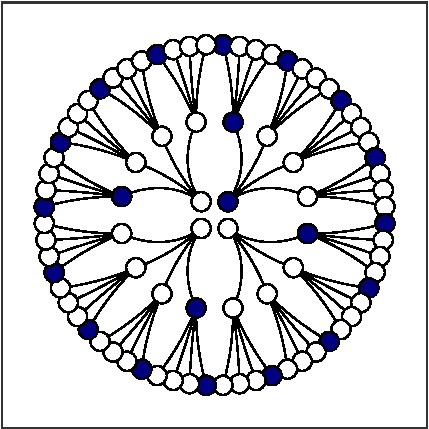
\includegraphics[width=0.33\linewidth]{unnamed-chunk-11-1} 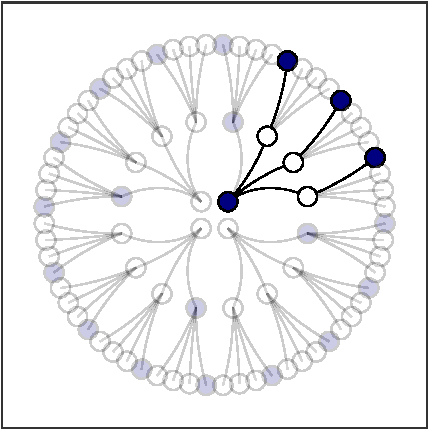
\includegraphics[width=0.33\linewidth]{unnamed-chunk-11-2} \end{figure}

Nur 3 der 64 \enquote{Pfade} (Kombinationen), die Hypothese {[}BWWW{]}
vorgibt, sind mit unseren Daten logisch zu vereinbaren.
\end{frame}

\begin{frame}{Kombinationen für Hypothesen}
\protect\hypertarget{kombinationen-fuxfcr-hypothesen}{}
\begin{tabular}{l|l}
\hline
Hypothese & Häufigkeit BWB\\
\hline
[W W W W] & 0 * 4 * 0 = 0\\
\hline
[B W W W] & 1 * 3 * 1 = 3\\
\hline
[B B W W] & 2 * 2 * 2 = 8\\
\hline
[B B B W] & 3 * 1 * 3 = 9\\
\hline
[B B B B] & 4 * 0 * 4 = 0\\
\hline
\end{tabular}

\begin{itemize}
\item
  Die Häufigkeiten der Kombinationen (Pfade) ist proportional zur
  Plausibilität einer Hypothese: Je mehr Pfade laut Hypothese, desto
  wahrscheinlicher die Hypothese (unter sonst gleichen Bedingungen).
\item
  Zusätzlich müssten wir noch beachten, ob bestimmte Hypothesen
  \emph{per se} bzw. \emph{a priori} wahrscheinlicher sind. So könnten
  blaue Murmeln selten sein. Gehen wir der Einfachheit halber zunächst
  davon aus, dass alle Hypothesen apriori gleich wahrscheinlich sind.
\end{itemize}
\end{frame}

\begin{frame}{Pfadbaum für die Hypothesen {[}BWWW{]}, {[}BBWW{]},
{[}BBBW{]}}
\protect\hypertarget{pfadbaum-fuxfcr-die-hypothesen-bwww-bbww-bbbw}{}
\begin{figure}[H]
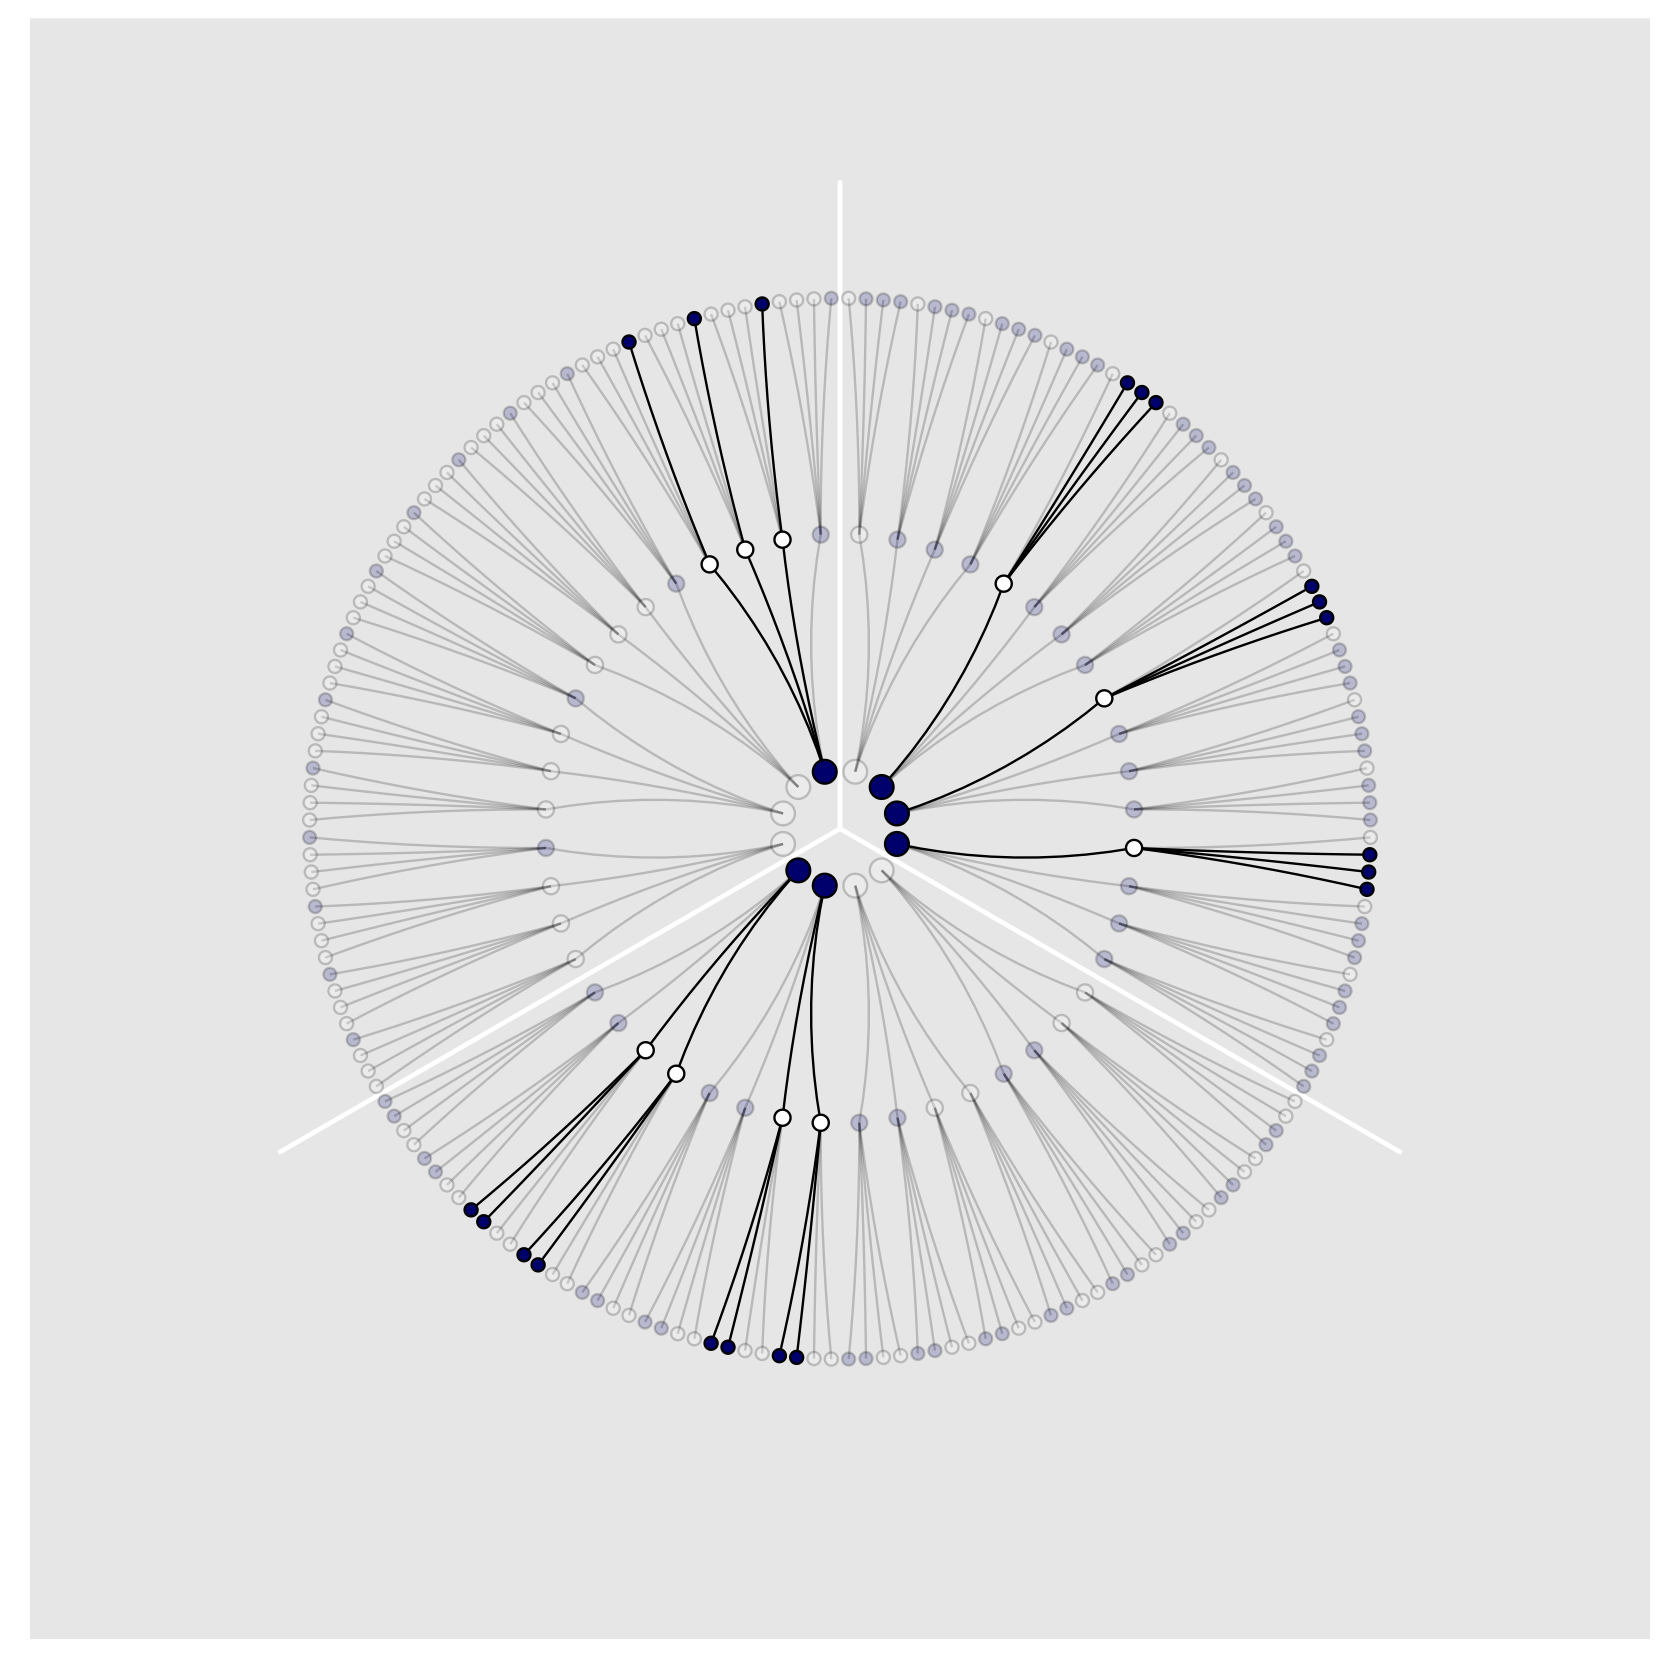
\includegraphics[width=0.7\linewidth]{/Users/sebastiansaueruser/github-repos/QM2-Folien/img/img2118} \end{figure}
\end{frame}

\begin{frame}{Wir ziehen einer vierte Murmel: B}
\protect\hypertarget{wir-ziehen-einer-vierte-murmel-b}{}
\begin{itemize}
\tightlist
\item
  Gehen wir zunächst davon aus, dass alle Hypothesen apriori gleich
  wahrscheinlich sind.
\item
  Wir ziehen wieder eine Murmel. Sie ist blau (B)!
\item
  Jetzt könnten wir den Pfadbaum für vier (statt drei) Züge aufmalen.
\item
  Oder wir machen ein \emph{Update}: Wir aktualisieren die bisherigen
  Kombinationshäufigkeiten um die neuen Daten. Die \emph{alten} Daten
  dienen dabei als \emph{Priori-Informationen} für die \emph{neuen}
  Daten.
\end{itemize}
\end{frame}

\begin{frame}{Priori-Information nutzen}
\protect\hypertarget{priori-information-nutzen}{}
Mit den Daten BWBB ist die Hypothese {[}BBBW{]} am wahrscheinlichsten:

\begin{tabular}[t]{l|r|r|l}
\hline
Hyp & PB & HA & HN\\
\hline
[W W W W] & 0 & 0 & 0 * 0 = 0\\
\hline
[B W W W] & 1 & 3 & 1 * 3 = 3\\
\hline
[B B W W] & 2 & 8 & 2 * 8 = 16\\
\hline
[B B B W] & 3 & 9 & 3 * 9 = 27\\
\hline
[B B B B] & 4 & 0 & 4 * 0 = 0\\
\hline
\end{tabular}

Hyp: Hypothese

PB: Anzahl von Pfaden für B

HA: alte (bisherige) Häufigkeiten

HN: neue (geupdatete) Häufigkeiten
\end{frame}

\begin{frame}{Murmelfabrik streikt: Blaue Murmeln jetzt sehr selten!}
\protect\hypertarget{murmelfabrik-streikt-blaue-murmeln-jetzt-sehr-selten}{}
\begin{itemize}
\item
  Berücksichtigen wir jetzt die Information, dass apriori (bevor wir die
  Daten gesehen haben), einige Hypothesen wahrscheinlicher (plausibler)
  sind als andere.
\item
  Hier ist die Hypothese {[}BBWW{]} am wahrscheinlichsten:
\end{itemize}

\begin{tabular}{l|r|r|l}
\hline
Hyp & HA & HF & HN\\
\hline
[W W W W] & 0 & 0 & 0 * 0 = 0\\
\hline
[B W W W] & 3 & 3 & 3 * 3 = 9\\
\hline
[B B W W] & 16 & 2 & 16 * 2 = 32\\
\hline
[B B B W] & 27 & 1 & 27 * 1 = 27\\
\hline
[B B B B] & 0 & 0 & 0 * 0 = 0\\
\hline
\end{tabular}

HF: Häufigkeit des Säckchentyps laut Fabrik.
\end{frame}

\begin{frame}{Zählen mit großen Zahlen nervt}
\protect\hypertarget{zuxe4hlen-mit-grouxdfen-zahlen-nervt}{}
\begin{itemize}
\item
  Malen Sie mal den Pfadbaum für 10 Züge \ldots{}
\item
  Eine Umrechnung der Häufigkeiten in \emph{Anteile} macht das Rechnen
  einfacher.
\item
  Dazu definieren wir die \emph{geupdatete Plausibilität einer Hypothese
  nach Kenntnis der Daten}:
\end{itemize}

\[\text{Plausibilität von [BWWW] nach Kenntnis von BWB}\] \[\propto\]
\[\text{Anzahl möglicher Pfade bei [BWWW] für BWB}\] \[\times\]
\[\text{Priori-Plausibilität von [BWWW]}\]

\begin{itemize}
\tightlist
\item
  \(\propto\): proportional zu
\end{itemize}
\end{frame}

\begin{frame}{Plausibilität berechnen}
\protect\hypertarget{plausibilituxe4t-berechnen}{}
\begin{itemize}
\tightlist
\item
  Sei \(p\) der Anteil blauer Murmeln. Bei Hypothese {[}BWWW{]} gilt,
  dann ist \(p=1/4 = 0.25\). Sei \(D_{neu} =\) BWB, die Daten:
\end{itemize}

\[\text{Plausibilität von }p\text{ nach Kenntnis von }D_{neu}\]
\[\propto\] \[\text{Anzahl Pfade von }p\text{ für }D_{neu}\] \[\times\]
\[\text{Priori-Plausibilität von }p\]

Für jeden Wert von \(p\) beurteilen wir dessen Plausibilität als umso
höher, je mehr Pfade durch den Pfadbaum führen und je höher die
Plausibilität des Werts von \(p\) von vornherein ist.
\end{frame}

\begin{frame}{Von Plausibilität zur Wahrscheinlichkeit}
\protect\hypertarget{von-plausibilituxe4t-zur-wahrscheinlichkeit}{}
\begin{itemize}
\tightlist
\item
  Teilen wir die Anzahl Pfade einer Hypothese durch die Anzahl aller
  Pfade (aller Hypothesen), so bekommen wir einen Anteil. Damit haben
  wir eine Wahrscheinlichkeit:
\end{itemize}

\[\text{Pl von }p\text{ mit Daten }D_{neu} =\]
\[\frac{\text{Anzahl Pfade von }p\text{ für }D_{neu}\times \text{Prior-Pl von }p}{\text{Summe aller Pfade}}\]

Pl: Plausibilität


\includegraphics[width=1em]{../img/weight.pdf} Was muss passieren, dass
der Bruch gleich Null ist?
\end{frame}

\begin{frame}[fragile]{Plausibilität pro Hypothese}
\protect\hypertarget{plausibilituxe4t-pro-hypothese}{}
\begin{tabular}{l|r|r|r}
\hline
Hyp & p & AP & Pl\\
\hline
[W W W W] & 0.00 & 0 & 0.00\\
\hline
[B W W W] & 0.25 & 3 & 0.15\\
\hline
[B B W W] & 0.50 & 8 & 0.40\\
\hline
[B B B W] & 0.75 & 9 & 0.45\\
\hline
[B B B B] & 1.00 & 0 & 0.00\\
\hline
\end{tabular}

p: Anteil blauer Murmeln (Priori-Wissen)

AP: Anzahl von möglichen Pfaden; Pl: Plausibilität

\begin{Shaded}
\begin{Highlighting}[]
\NormalTok{AP }\OtherTok{\textless{}{-}} \FunctionTok{c}\NormalTok{(}\DecValTok{0}\NormalTok{, }\DecValTok{3}\NormalTok{, }\DecValTok{8}\NormalTok{, }\DecValTok{9}\NormalTok{, }\DecValTok{0}\NormalTok{)}
\NormalTok{Pl }\OtherTok{\textless{}{-}}\NormalTok{ AP }\SpecialCharTok{/} \FunctionTok{sum}\NormalTok{(AP)}
\NormalTok{Pl}
\end{Highlighting}
\end{Shaded}

\begin{verbatim}
## [1] 0.00 0.15 0.40 0.45 0.00
\end{verbatim}
\end{frame}

\begin{frame}{Fachbegriffe}
\protect\hypertarget{fachbegriffe}{}
\begin{itemize}
\item
  Kennwerte laut einer Hypothese, wie den Anteil blauer Murmeln \(p\)
  bezeichnet man als \emph{Parameter}.
\item
  Den Anteil gültiger Pfade pro Hypothese (bzw. pro Wert von \(p\))
  bezeichnet man als \emph{Likelihood}.
\item
  Die Priori-Plausibilität nennt man \emph{Priori-Wahrscheinlichkeit}.
\item
  Die neue, geupdatete Plausibilität für einen bestimmten Wert von \(p\)
  nennt man \emph{Posteriori-Wahrscheinlichkeit}.
\end{itemize}


\includegraphics[width=1em]{../img/weight.pdf} Erklären Sie die Begriffe
dem nächsten Menschen, den Sie treffen!
\end{frame}

\begin{frame}{Zusammenfassung}
\protect\hypertarget{zusammenfassung}{}
\begin{enumerate}
\item
  Schritt: Unser Vorab-Wissen zur Wahrscheinlichkeit jeder Hypothese
  wird mit dem Begriff \emph{Priori-Verteilung} gefasst.
\item
  Schritt: Wir zählen den Anteil gültiger Pfade für jede Hypothese; d.h.
  wir berechnen den \emph{Likelihood} jeder Hypothese.
\item
  Schritt: Mit den Likelihoods \emph{updaten} wir unsere
  Priori-Verteilung. Die Wahrscheinlichkeit jeder Hypothese verändert
  sich entsprechend der Daten. Es resultiert die
  \emph{Posteriori-Verteilung}.
\end{enumerate}
\end{frame}

\hypertarget{ein-erstes-modell}{%
\section{Ein erstes Modell}\label{ein-erstes-modell}}

\begin{frame}{Welcher Anteil der Erdoberfläche ist mit Wasser bedeckt?}
\protect\hypertarget{welcher-anteil-der-erdoberfluxe4che-ist-mit-wasser-bedeckt}{}
\begin{columns}[T]
\begin{column}{0.3\textwidth}
\begin{figure}[H]

\includegraphics[width=0.7\linewidth]{/Users/sebastiansaueruser/github-repos/QM2-Folien/img/earth} \end{figure}
\tiny

\href{https://pngimg.com/image/25340}{Quelle} CC 4.0 BY-NC \normalsize
\end{column}

\begin{column}{0.7\textwidth}
Sie werden einen Globus-Ball in die Luft und fangen in wieder auf. Sie
notieren dann, ob die Stelle unter Ihrem Zeigefinger Wasser zeigt (W)
oder Land (L). Den Versuch wiederholen Sie 9 Mal.
\end{column}
\end{columns}

\[W \quad L \quad W \quad W \quad W \quad L \quad W \quad L \quad W\]


\includegraphics[width=1em]{../img/weight.pdf} Besorgen Sie sich einen
Globus (zur Not eine Münze) und stellen Sie den Versuch nach!
\end{frame}

\begin{frame}{Der datengenierende Prozess: Wie entstanden die Daten?}
\protect\hypertarget{der-datengenierende-prozess-wie-entstanden-die-daten}{}
\begin{enumerate}
\tightlist
\item
  Der wahre Anteil von Wasser der Erdoberfläche ist \(p\).
\item
  Ein Wurf des Globusballes hat die Wahrscheinlichkeit \(p\), eine
  \(W\)-Beobachtung zu erzeugen.
\item
  Die Würfe des Globusballes sind unabhängig voneinander.
\item
  Wir haben kein Vorwissen über \(p\); jeder Wert ist uns gleich
  wahrscheinlich.
\end{enumerate}


\includegraphics[width=1em]{../img/weight.pdf} Welche Annahmen würden
Sie ändern? Welche könnte man wegnehmen? Welche hinzufügen? Was wären
die Konsequenzen?
\end{frame}

\begin{frame}{Wissen updaten: Wir füttern Daten in das Modell}
\protect\hypertarget{wissen-updaten-wir-fuxfcttern-daten-in-das-modell}{}
\begin{figure}[H]
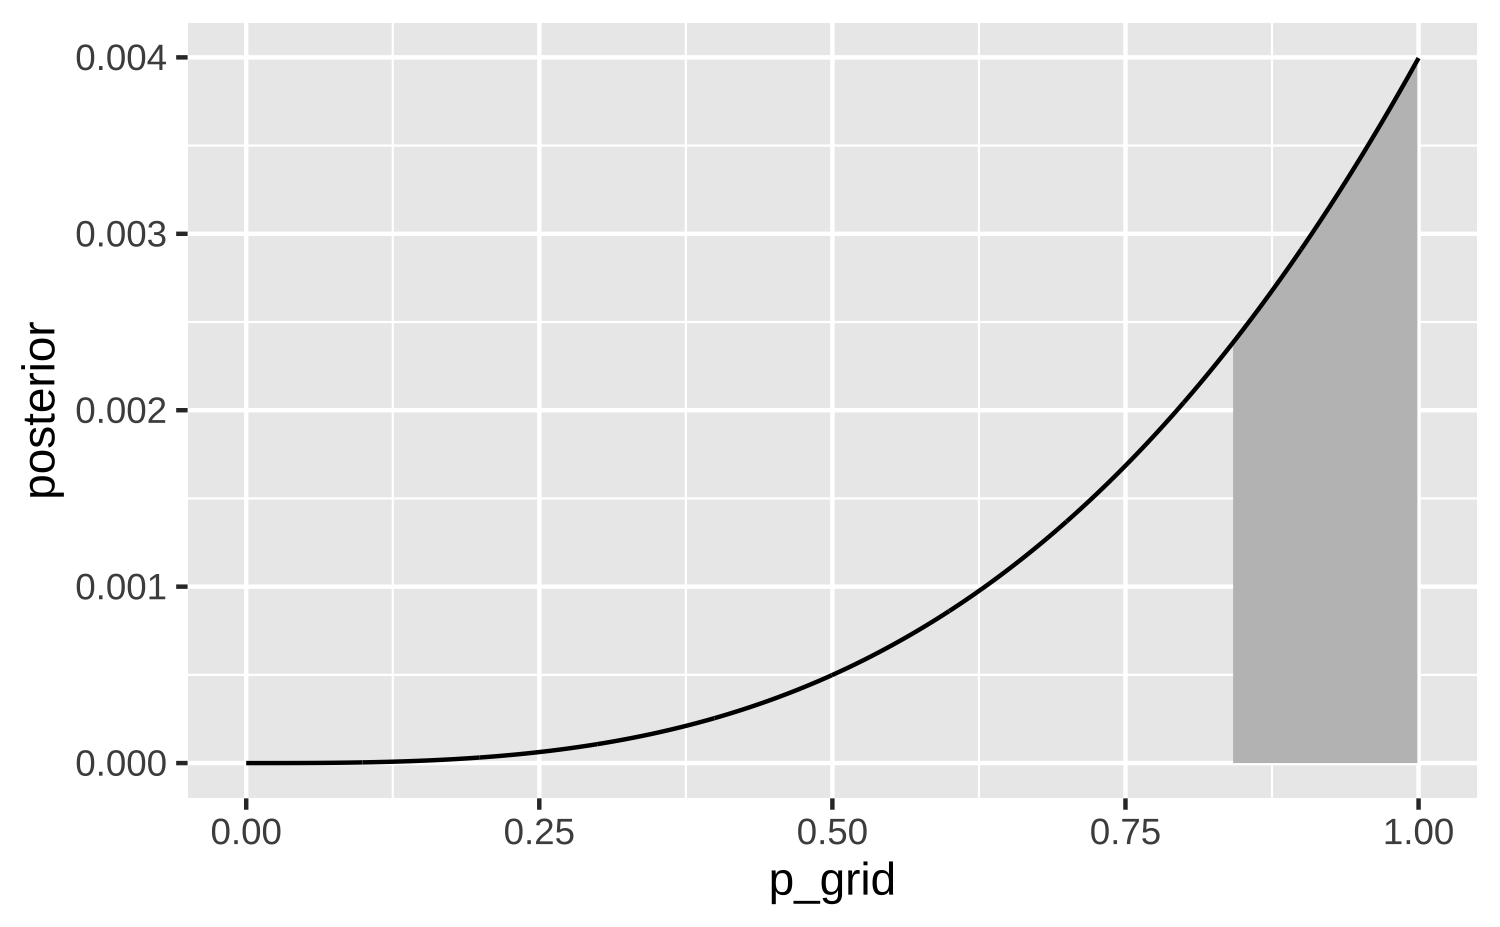
\includegraphics[width=1\linewidth]{unnamed-chunk-19-1} \end{figure}
\end{frame}

\begin{frame}{Erinnern wir uns an das Urnen-Beispiel}
\protect\hypertarget{erinnern-wir-uns-an-das-urnen-beispiel}{}
\begin{itemize}
\item
  Für jede Hypothese haben wir ein Vorab-Wissen, das die jeweilige
  Plausibilität der Hypothese angibt: \emph{Priori-Verteilung}.
\item
  Für jede Hypothese (d.h. jeden \emph{Parameterwert} \(p\)) möchten wir
  den Anteil (die Wahrscheinlichkeit) gültiger Kombinationen wissen. Das
  gibt uns den \emph{Likelihood}.
\item
  Dann gewichten wir den Likelihood mit dem Vorabwissen, so dass wir die
  \emph{Posteriori-Verteilung}\footnote<.->{Anstatt von \emph{Priori}
    liest man auch \emph{Prior}; anstatt \emph{Posteriori} auch
    \emph{Posterior}} bekommen.
\end{itemize}

\begin{figure}[H]

\includegraphics[width=0.7\linewidth]{/Users/sebastiansaueruser/github-repos/QM2-Folien/img/bayesupdate} \end{figure}
\end{frame}

\begin{frame}{Die Binomialverteilung}
\protect\hypertarget{die-binomialverteilung}{}
Wir nehmen an, dass die Daten unabhängig voneinander entstehen und sich
der Parameterwert nicht zwischenzeitlich ändert.

Dann kann man die Wahrscheinlichkeit (\(Pr\)), \(W\) mal Wasser und
\(L\) mal Land zu beobachten, wenn die Wahrscheinlichkeit für Wasser
\(p\) beträgt, mit der \emph{Binomialverteilung} berechnen.

Die Binomialverteilung zeigt die Verteilung der Häufigkeit
(Wahrscheinlichkeit) der Ereignisse (z.B. 2 Mal Kopf) beim wiederholten
Münzwurf (und allen vergleichbaren Zufallsexperimenten)\footnote<.->{\enquote{Münzwurfverteilung}}.

\[Pr(W,L|p) = \frac{(W+L)!}{W!L!}p^W(1-p)^L\]
\end{frame}

\begin{frame}[fragile]{Binomialverteilung mit R}
\protect\hypertarget{binomialverteilung-mit-r}{}
Was ist der Anteil der gültigen Pfade (Wahrscheinlichkeit), um 6 mal
\(W\) bei \(N=W+L=9\) Würfen zu bekommen, wenn wir von \(p=1/2\)
ausgehen?

\begin{Shaded}
\begin{Highlighting}[]
\FunctionTok{dbinom}\NormalTok{(}\AttributeTok{x =} \DecValTok{6}\NormalTok{, }\AttributeTok{size =} \DecValTok{9}\NormalTok{, }\AttributeTok{prob =} \DecValTok{1}\SpecialCharTok{/}\DecValTok{2}\NormalTok{)}
\end{Highlighting}
\end{Shaded}

\begin{verbatim}
## [1] 0.1640625
\end{verbatim}

Was ist die Wahrscheinlichkeit für \(W=9\) bei \(N=9\) und \(p=1/2\)?

\begin{Shaded}
\begin{Highlighting}[]
\FunctionTok{dbinom}\NormalTok{(}\AttributeTok{x =} \DecValTok{9}\NormalTok{, }\AttributeTok{size =} \DecValTok{9}\NormalTok{, }\AttributeTok{prob =} \DecValTok{1}\SpecialCharTok{/}\DecValTok{2}\NormalTok{)}
\end{Highlighting}
\end{Shaded}

\begin{verbatim}
## [1] 0.001953125
\end{verbatim}
\end{frame}

\begin{frame}[fragile]{Beispiele zur Berechnung einer binomial
verteilten Wahrscheinlichkeit}
\protect\hypertarget{beispiele-zur-berechnung-einer-binomial-verteilten-wahrscheinlichkeit}{}
Ei Professori stellt einen Klausur mit 20 Richtig-Falsch-Fragen. Wie
groß ist die Wahrscheinlichkeit, durch bloßes Münze werfen genau 15
Fragen richtig zu raten?\footnote<.->{Hey, endlich mal was für echte
  Leben!}

\begin{Shaded}
\begin{Highlighting}[]
\FunctionTok{dbinom}\NormalTok{(}\AttributeTok{x =} \DecValTok{15}\NormalTok{, }\AttributeTok{size =} \DecValTok{20}\NormalTok{, }\AttributeTok{prob =}\NormalTok{ .}\DecValTok{5}\NormalTok{)}
\end{Highlighting}
\end{Shaded}

\begin{verbatim}
## [1] 0.01478577
\end{verbatim}

Was ist die Wahrscheinlichkeit bei 3 Münzwürfen (genau) 3 Treffer (Kopf)
zu erzielen?

\begin{Shaded}
\begin{Highlighting}[]
\FunctionTok{dbinom}\NormalTok{(}\DecValTok{3}\NormalTok{, }\DecValTok{3}\NormalTok{, }\DecValTok{1}\SpecialCharTok{/}\DecValTok{2}\NormalTok{)}
\end{Highlighting}
\end{Shaded}

\begin{verbatim}
## [1] 0.125
\end{verbatim}
\end{frame}

\begin{frame}{Unser Modell ist geboren}
\protect\hypertarget{unser-modell-ist-geboren}{}
Wir fassen das Globusmodell so zusammen:

\[W \sim \text{Bin}(N,p),\]

Lies: \enquote{W ist \emph{bin}omial verteilt mit den Parametern \(N\)
und \(p\)}. \(N\) gibt die Anzahl der Globuswürfe an: \(N=W+L\).

Unser Vorab-Wissen zu \(p\) sei, dass uns alle Werte gleich plausibel
erscheinen (\enquote{uniform}):

\[p \sim \text{Unif}(0,1).\]

Lies: \enquote{\(p\) ist gleich (uniform) verteilt mit der Untergrenze 0
und der Obergrenze 1}.
\end{frame}

\begin{frame}{So sehen die Verteilungen aus}
\protect\hypertarget{so-sehen-die-verteilungen-aus}{}
\begin{columns}[T]
\begin{column}{0.5\textwidth}
\begin{block}{Binomialverteilung}
\protect\hypertarget{binomialverteilung}{}
\begin{figure}[H]
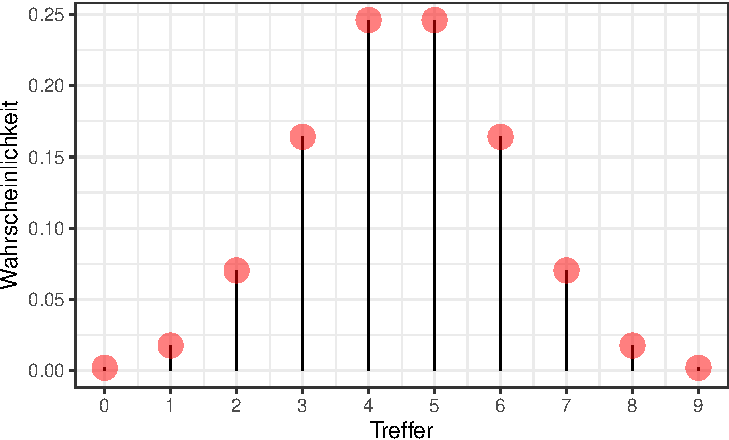
\includegraphics[width=0.7\linewidth]{unnamed-chunk-25-1} \end{figure}

\(N=9, p = 1/2\)
\end{block}
\end{column}

\begin{column}{0.5\textwidth}
\begin{block}{Gleichverteilung}
\protect\hypertarget{gleichverteilung}{}
\begin{figure}[H]
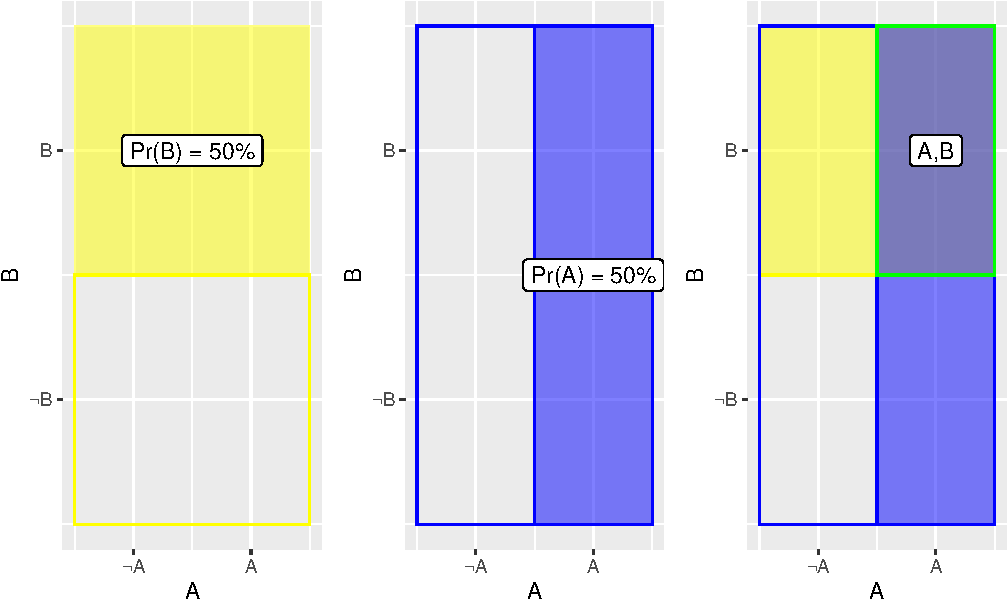
\includegraphics[width=0.7\linewidth]{unnamed-chunk-26-1} \end{figure}

\(Min = 0, Max = 1\)
\end{block}
\end{column}
\end{columns}


\includegraphics[width=1em]{../img/weight.pdf} Was fällt Ihnen bei der
Binomialverteilung auf? Ist sie symmetrisch? Verändert sich die
Wahrscheinlichkeit linear? Was fällt Ihnen bei der Gleichverteilung auf?
\end{frame}

\begin{frame}{Herleitung Bayes' Theorem 1/2: Gemeinsame
Wahrscheinlichkeit}
\protect\hypertarget{herleitung-bayes-theorem-12-gemeinsame-wahrscheinlichkeit}{}
Die Wahrscheinlichkeit für \emph{Regen} und \emph{kalt} ist gleich der
Wahrscheinlihckeit von \emph{Regen}, \emph{gegeben kalt} mal der
Wahrscheinlicht von \emph{kalt}. Entsprechend gilt: Die
Wahrscheinlichkeit von \(W\), \(L\) und \(p\) ist das Produkt von
\(Pr(W,L|p)\) und der Prior-Wahrscheinlichkeit \(Pr(p)\):

\[Pr(W,L,p) = Pr(W,L|p) \cdot Pr(p)\]

Genauso gilt: Die Wahrscheinlichkeit von \emph{Regen} und \emph{kalt}
ist gleich der Wahrscheinlichkeit \emph{kalt, wenn's regnet} mal der
Wahrscheinlichkeit von \emph{Regen}:

\[Pr(W,L,p) = Pr(p|W,L) \cdot Pr(W, L)\]
\end{frame}

\begin{frame}{Herleitung Bayes' Theorem 2/2:
Posteriori-Wahrscheinlichkeit}
\protect\hypertarget{herleitung-bayes-theorem-22-posteriori-wahrscheinlichkeit}{}
Wir setzen die letzten beiden Gleichungen gleich:

\[Pr(W,L|p) \cdot Pr(p) = Pr(p|W,L) \cdot (W,L)\]

Und lösen auf nach der Posteriori-Wahrscheinlichkeit, \(Pr(p|W,L)\):

\[Pr(p|W,L) = \frac{Pr(W,L|p) Pr(p)}{Pr(W,L)}\]

\(Pr(W,L)\) nennt man die \emph{mittlere Wahrscheinlichkeit der Daten}
oder \emph{Evidenz}. Die Evidenz berechnet sich als Mittelwert der
Likelihoods über alle Werte von \(p\). Die Aufgabe dieser Größe ist nur
dafür zu sorgen, dass insgesamt Werte zwischen 0 und 1 herauskommen.
\end{frame}

\begin{frame}{Bayes' Theorem}
\protect\hypertarget{bayes-theorem}{}
\begin{alertblock}{Formel Bayes' Theorem}
$$Pr(H|D) = \frac{Pr(D|H) Pr(H)}{Pr(D)}$$
\end{alertblock}

\begin{itemize}
\item
  Bestandteile:

  \begin{itemize}
  \item
    Posteriori-Wahrscheinlichkeit: \(Pr_{Post} := Pr(H|D)\)
  \item
    Likelihood: \(L := Pr(D|H)\)
  \item
    Priori-Wahrscheinlichkeit: \(Pr_{Priori} := Pr(H)\)
  \item
    Evidenz: \(E := Pr(D)\)
  \end{itemize}
\item
  Bayes' Theorem gibt die \(Pr_{Post}\) an, wenn man die Gleichung mit
  der \(Pr_{Priori}\) und dem \(L\) füttert.
\item
  Bayes' Theorem wird häufig verwendet, um die \(Pr_{Post}\) zu
  quantifizieren.
\item
  Die \(Pr_{Post}\) ist proportional zu \(L \times Pr_{Priori}\).
\end{itemize}
\end{frame}

\begin{frame}{Posteriori als Produkt von Priori und Likelihood}
\protect\hypertarget{posteriori-als-produkt-von-priori-und-likelihood}{}
\[\text{Posteriori} = \frac{\text{Likelihood} \times \text{Priori}}{\text{Evidenz}}\]

\begin{figure}[H]
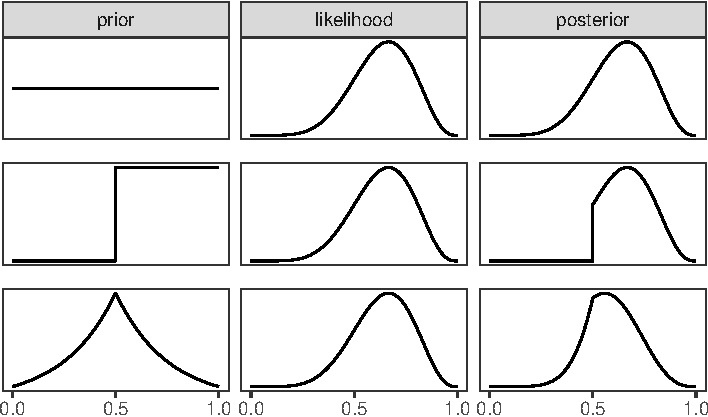
\includegraphics[width=0.7\linewidth]{unnamed-chunk-27-1} \end{figure}
\end{frame}

\hypertarget{bayes-berechnen-mit-r}{%
\section{Bayes berechnen mit R}\label{bayes-berechnen-mit-r}}

\begin{frame}{Die Methode \emph{Gitter-Annäherung}\footnote<.->{Grid
  Approximation}}
\protect\hypertarget{die-methode-gitter-annuxe4herung}{}
\begin{enumerate}
\tightlist
\item
  Teile den Wertebereich des Parameter in ein \enquote{Gitter} auf, z.B.
  \(0.1, 0.2, ..., 0.9, 1\) (\enquote{Gitterwerte}).
\item
  Bestimme den Priori-Wert des Parameters für jeden Gitterwert.
\item
  Berechne den Likelihood für Gitterwert.
\item
  Berechne den unstandardisierten Posteriori-Wert für jeden Gitterwert
  (Produkt von Priori und Likelihood).
\item
  Standardisiere den Posteriori-Wert durch teilen anhand der Summe alle
  unstand. Posteriori-Werte.
\end{enumerate}
\end{frame}

\begin{frame}[fragile]{Gitterwerte in R berechnen}
\protect\hypertarget{gitterwerte-in-r-berechnen}{}
\footnotesize

\begin{Shaded}
\begin{Highlighting}[]
\NormalTok{d }\OtherTok{\textless{}{-}}
  \FunctionTok{tibble}\NormalTok{(}
    \CommentTok{\# definiere das Gitter: }
    \AttributeTok{p\_Gitter =} \FunctionTok{seq}\NormalTok{(}\AttributeTok{from =} \DecValTok{0}\NormalTok{, }\AttributeTok{to =} \DecValTok{1}\NormalTok{, }\AttributeTok{length.out =} \DecValTok{10}\NormalTok{),}
    \CommentTok{\# bestimme den Priori{-}Wert:       }
    \AttributeTok{Priori  =} \DecValTok{1}\NormalTok{) }\SpecialCharTok{\%\textgreater{}\%}  
    \FunctionTok{mutate}\NormalTok{(}
      \CommentTok{\# berechne Likelihood für jeden Gitterwert:}
      \AttributeTok{Likelihood =} \FunctionTok{dbinom}\NormalTok{(}\DecValTok{6}\NormalTok{, }\AttributeTok{size =} \DecValTok{9}\NormalTok{, }\AttributeTok{prob =}\NormalTok{ p\_Gitter),}
      \CommentTok{\# berechen unstand. Posteriori{-}Werte:}
      \AttributeTok{unstd\_Post =}\NormalTok{ Likelihood }\SpecialCharTok{*}\NormalTok{ Priori,}
      \CommentTok{\# berechne stand. Posteriori{-}Werte (summiert zu 1):}
      \AttributeTok{Post =}\NormalTok{ unstd\_Post }\SpecialCharTok{/} \FunctionTok{sum}\NormalTok{(unstd\_Post))  }
\end{Highlighting}
\end{Shaded}

\normalsize
\end{frame}

\begin{frame}{Unsere Gitter-Daten}
\protect\hypertarget{unsere-gitter-daten}{}
\begin{tabular}[t]{r|r|r|r|r}
\hline
p\_Gitter & Priori & Likelihood & unstd\_Post & Post\\
\hline
0.00 & 1 & 0.00 & 0.00 & 0.00\\
\hline
0.11 & 1 & 0.00 & 0.00 & 0.00\\
\hline
0.22 & 1 & 0.00 & 0.00 & 0.01\\
\hline
0.33 & 1 & 0.03 & 0.03 & 0.04\\
\hline
0.44 & 1 & 0.11 & 0.11 & 0.12\\
\hline
0.56 & 1 & 0.22 & 0.22 & 0.24\\
\hline
0.67 & 1 & 0.27 & 0.27 & 0.30\\
\hline
0.78 & 1 & 0.20 & 0.20 & 0.23\\
\hline
0.89 & 1 & 0.06 & 0.06 & 0.06\\
\hline
1.00 & 1 & 0.00 & 0.00 & 0.00\\
\hline
\end{tabular}


\includegraphics[width=1em]{../img/weight.pdf} Was wohl mit \emph{Post}
passiert, wenn wir \emph{Priori} ändern?
\end{frame}

\begin{frame}{\(Pr_{Post}\) zeigt, wie plausibel wir jeden Wert von
\(p\) halten}
\protect\hypertarget{pr_post-zeigt-wie-plausibel-wir-jeden-wert-von-p-halten}{}
\begin{figure}[H]
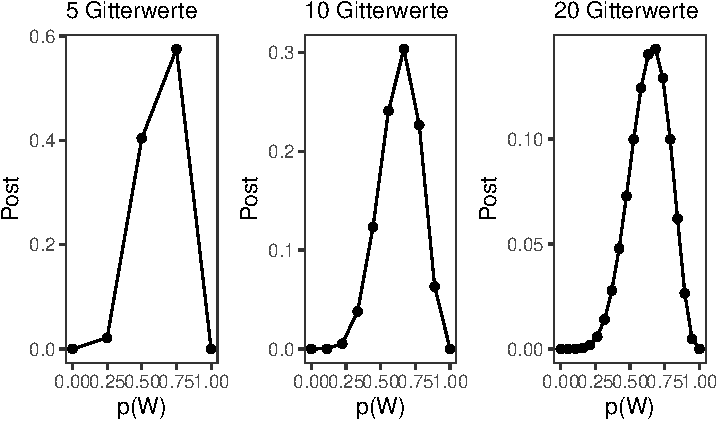
\includegraphics[width=1\linewidth]{unnamed-chunk-30-1} \end{figure}

Mehr Gitterwerte glätten die Annäherung.
\end{frame}

\begin{frame}[fragile]{Quadratische Anpassung\footnote<.->{Quadratic
  Approximation}}
\protect\hypertarget{quadratische-anpassung}{}
\begin{itemize}
\item
  Komfortabler noch ist die \emph{quadratische Anpassung}, die bestimmte
  statistische Eigenschaften von linearen Modellen ausnutzt.
\item
  Der R-Befehl \texttt{quap} gibt zentrale Statistiken zu den Parametern
  des Modells zurück.
\end{itemize}

\tiny

\begin{Shaded}
\begin{Highlighting}[]
\FunctionTok{library}\NormalTok{(rethinking)}

\NormalTok{globus\_qa }\OtherTok{\textless{}{-}} \FunctionTok{quap}\NormalTok{(  }\CommentTok{\# "quadratic approximation"}
  \FunctionTok{alist}\NormalTok{(  }\CommentTok{\# definiere die Modellgleichungen}
\NormalTok{    W }\SpecialCharTok{\textasciitilde{}} \FunctionTok{dbinom}\NormalTok{(W }\SpecialCharTok{+}\NormalTok{ L, p),  }\CommentTok{\# Likelihood ist binomial verteilt}
\NormalTok{    p }\SpecialCharTok{\textasciitilde{}} \FunctionTok{dunif}\NormalTok{(}\DecValTok{0}\NormalTok{, }\DecValTok{1}\NormalTok{)        }\CommentTok{\# Priori ist gleich (uniform) verteilt}
\NormalTok{  ), }
  \AttributeTok{data =} \FunctionTok{list}\NormalTok{(}\AttributeTok{W =} \DecValTok{6}\NormalTok{, }\AttributeTok{L =} \DecValTok{3}\NormalTok{)  }\CommentTok{\# Daten}
\NormalTok{)}


\FunctionTok{precis}\NormalTok{(globus\_qa)  }\CommentTok{\# Gibt uns die zentralen Ergebnisse}
\end{Highlighting}
\end{Shaded}

\begin{verbatim}
##        mean        sd      5.5%     94.5%
## p 0.6666667 0.1571338 0.4155366 0.9177968
\end{verbatim}

\normalsize
\end{frame}

\begin{frame}{Je größer die Stichprobe (\(N\)), desto zuverlässiger wird
unsere Berechnung}
\protect\hypertarget{je-gruxf6uxdfer-die-stichprobe-n-desto-zuverluxe4ssiger-wird-unsere-berechnung}{}
\begin{figure}[H]
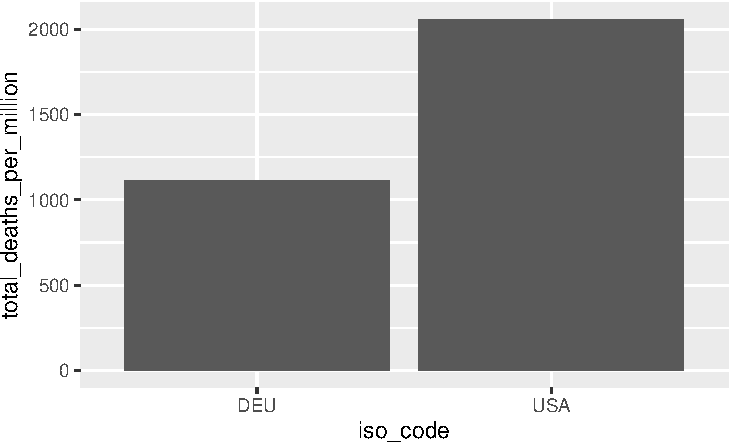
\includegraphics[width=1\linewidth]{unnamed-chunk-32-1} \end{figure}

Grau: Quadratische Anpassung; schwarz: wahre Verteilung
\end{frame}

\begin{frame}{Zusammenfassung}
\protect\hypertarget{zusammenfassung-1}{}
\begin{itemize}
\item
  In unserem Modell haben wir Annahmen zu \(Pr_{Priori}\) und \(L\)
  getroffen.
\item
  Auf dieser Basis hat der Golem sein Wissen geupdated zu \(Pr_{Post}\).
\item
  Mit der Gitter-Methode haben wir viele Hypothesen (Parameterwerte)
  untersucht und jeweils die \(Pr_{Post}\) berechnet.
\item
  Unser Modell bildet die kleine Welt ab; ob es in der großen Welt
  nützlich ist, steht auf einem anderen Blatt.
\end{itemize}


\includegraphics[width=1em]{../img/weight.pdf} Wenn Sie auf einen
Prozentwert für \(W\) tippen müssten, welchen würden Sie nehmen, laut
dem Modell (und gegeben der Daten)?
\end{frame}

\hypertarget{hinweise}{%
\section{Hinweise}\label{hinweise}}

\begin{frame}{Hinweise zum Skript}
\protect\hypertarget{hinweise-zum-skript}{}
Dieses Skript bezieht sich auf folgende
\protect\hyperlink{literatur}{Lehrbücher}:

\begin{itemize}
\tightlist
\item
  Kapitel 2 aus McElreath (2020)
\item
  R-Code für die Diagramme stammt aus Kurz (2021)
\end{itemize}

Dieses Skript wurde erstellt am 2021-10-06 11:03:04.
\end{frame}

\begin{frame}{Literatur}
\protect\hypertarget{literatur}{}
\hypertarget{refs}{}
\begin{CSLReferences}{1}{0}
\leavevmode\vadjust pre{\hypertarget{ref-kurz_statistical_2021}{}}%
Kurz, A. Solomon. 2021. \emph{Statistical Rethinking with Brms, Ggplot2,
and the Tidyverse: {Second} Edition}.
\url{https://bookdown.org/content/4857/}.

\leavevmode\vadjust pre{\hypertarget{ref-mcelreath_statistical_2020}{}}%
McElreath, Richard. 2020. \emph{Statistical Rethinking: A {Bayesian}
Course with Examples in {R} and {Stan}}. 2. Aufl. {CRC} Texts in
Statistical Science. {Boca Raton}: {Taylor and Francis, CRC Press}.

\end{CSLReferences}
\end{frame}

\end{document}
